\begin{frame}{Generative Learning}

  What's generative learning?

\end{frame}

\begin{frame}{Generative Learning}

  We want to model the data distribution $p(x)$ directly.

  \note{
    \begin{itemize}
      \item Where $x$ is a sample image.
      \item How is this even possible? Let's see ...
    \end{itemize}
  }

\end{frame}


\begin{frame}{PixelRNN/PixelCNN}

  \begin{align*}
    p(x) = p(x_{1}, ..., x_{n}) = \prod_{i}^{n^{2}} p(x_{i})p(x_{i}|x_{1}, ..., x_{i-1})
  \end{align*}

  \begin{figure}
    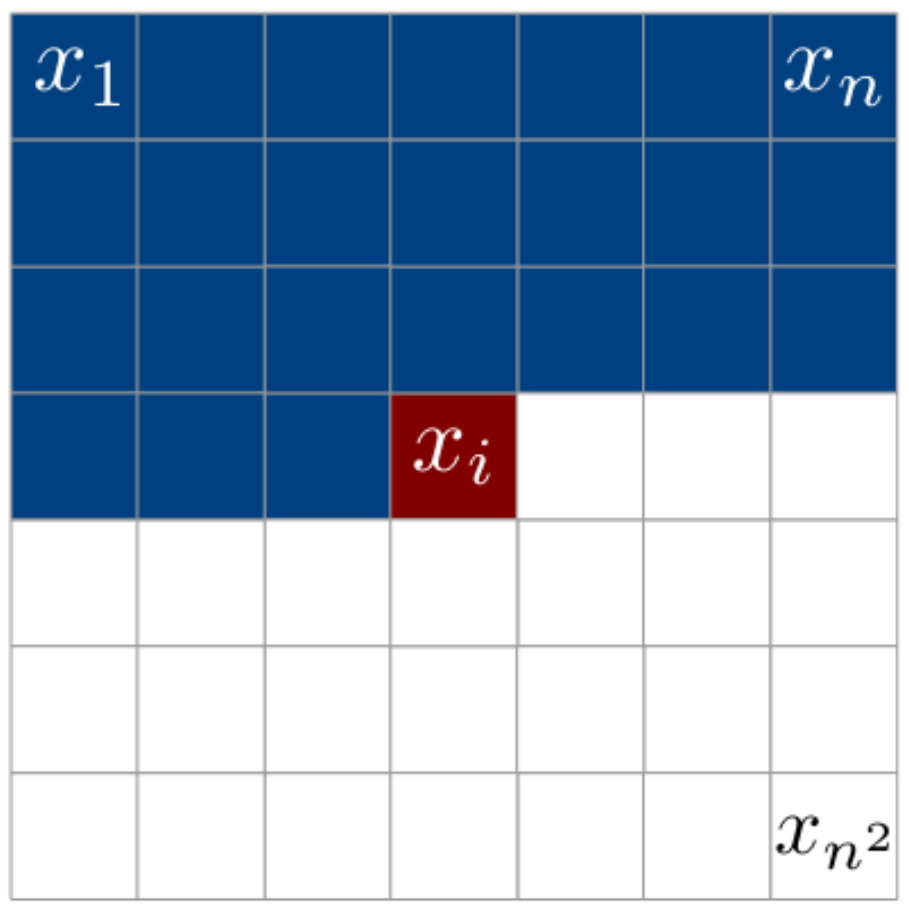
\includegraphics[width=0.3\textwidth]{pixelrnn_pixels}
  \end{figure}

  \note{
    \begin{itemize}
      \item Fully Visible Belief Network
      \item Product of distributions using chain rule (decompose likelihood of an image into pixel probabilities).
      \item Train RNN to classify pixels (e.g. 1 out of 255).
      \item Also possible to formulate as CNN, but still one forward pass per pixel necessary at test time.
      \item Image from Pixel Recurrent Neural Networks, van den Oord, ICML 2016
    \end{itemize}
  }
\end{frame}


\begin{frame}{Modeling using a latent variable}

  \begin{columns}
    \hspace{2cm}
    \begin{column}{0.3\textwidth}
      \begin{align*}
        z = \begin{pmatrix}
          haircolor \\
          skin tone \\
          beard \\
          gender \\
          classes \\
          expression
        \end{pmatrix}
      \end{align*}
    \end{column}
    \begin{column}{0.1\textwidth}
      \begin{align*}
        \Rightarrow
      \end{align*}
    \end{column}
    \begin{column}{0.4\textwidth}
      \begin{figure}
        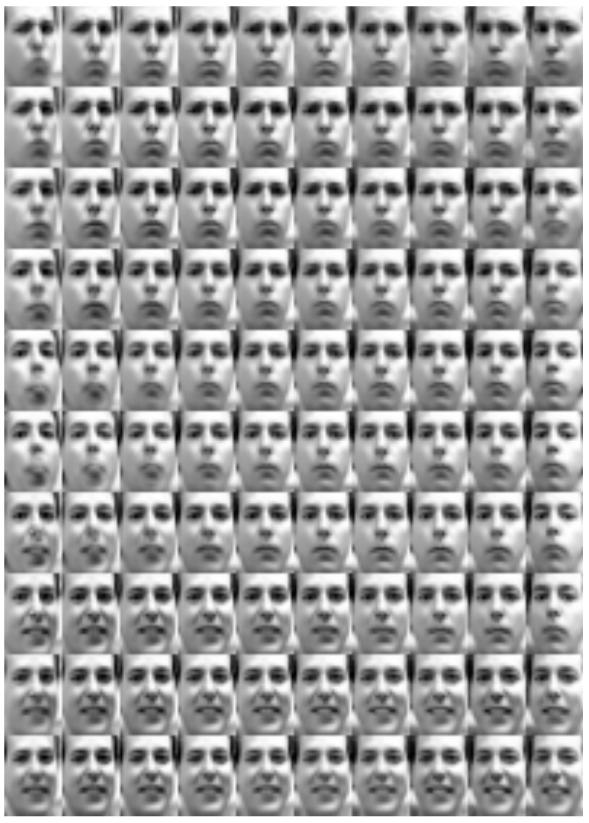
\includegraphics[width=.6\textwidth]{vae_faces}
      \end{figure}
    \end{column}
    \hspace{2cm}
  \end{columns}

  \note{
    \begin{itemize}
      \item Image from Auto-Encoding Variational Bayes, Kingma \& Welling, ICLR 2014
      \item
    \end{itemize}
  }

\end{frame}


\begin{frame}{Modeling using a latent variable}

  \begin{align*}
    p_{\theta}(x) = \int p_{\theta}(x|z)p_{\theta}(z) dz
  \end{align*}

  \begin{columns}
    \hspace{2cm}
    \begin{column}{0.3\textwidth}
      \begin{align*}
        z = \begin{pmatrix}
          haircolor \\
          skin tone \\
          beard \\
          gender \\
          classes \\
          expression
        \end{pmatrix}
      \end{align*}
    \end{column}
    \begin{column}{0.1\textwidth}
      \begin{align*}
        \Rightarrow
      \end{align*}
    \end{column}
    \begin{column}{0.4\textwidth}
      \begin{figure}
        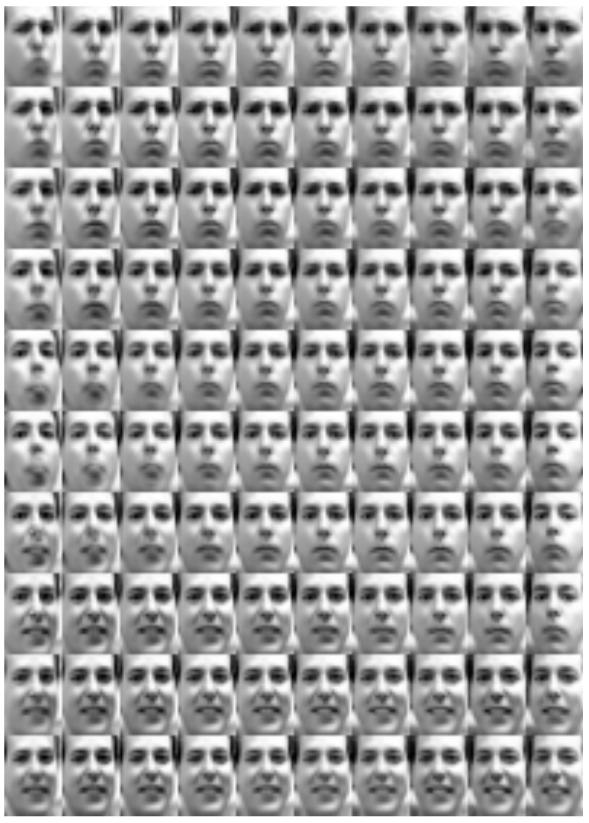
\includegraphics[width=.6\textwidth]{vae_faces}
      \end{figure}
    \end{column}
    \hspace{2cm}
  \end{columns}

  \note{
    \begin{itemize}
      \item $p_{\theta}$ is the data likelihood we want to maximize.
      \item We can approximate $p(z)$ e.g. as Gaussian.
      \item We can learn $p(x|z)$ e.g. with a generator network.
      \item However, the integral over $z$ is intractable.
    \end{itemize}
  }

\end{frame}


\begin{frame}{ELBO (evidence lower bound)}

  \begin{align*}
    E_{q(z|x)} \log p(x|z) - KL(q(z|x)||p(z))
  \end{align*}

  \note{
    \begin{itemize}
      \item Luckily it turns out that this term is a lower bound on our intractable data likelihood.
      \item $KL$ is the Kullback-Leibler divergence, a similarity measurement for probability distributions.
      \item $q(z|x)$ is a tractable approximation of the intractable $p(z|x)$.
      \item Yes, there is a lot of math we just skipped. You can find a full derivation here: \url{https://www.youtube.com/watch?v=uaaqyVS9-rM&t=1182s}
    \end{itemize}
  }

\end{frame}


\begin{frame}{ELBO (evidence lower bound)}

  \begin{align*}
    E_{q(z|x)} \log p(x|z) - KL(q(z|x)||p(z))
  \end{align*}

  \vspace{2cm}

  \center{\huge{Let's maximize it!}}

  \note{
    \begin{itemize}
      \item Luckily it turns out that this term is a lower bound on our intractable data likelihood.
      \item $KL$ is the Kullback-Leibler divergence, a similarity measurement for probability distributions.
      \item $q(z|x)$ is a tractable approximation of the intractable $p(z|x)$.
    \end{itemize}
  }

\end{frame}


\begin{frame}{Variational Autoencoder (VAE)}

  \begin{align*}
    q(z|x) = \mathcal{N}(\mu_{z}, \sigma_{z})
  \end{align*}

  \begin{figure}
    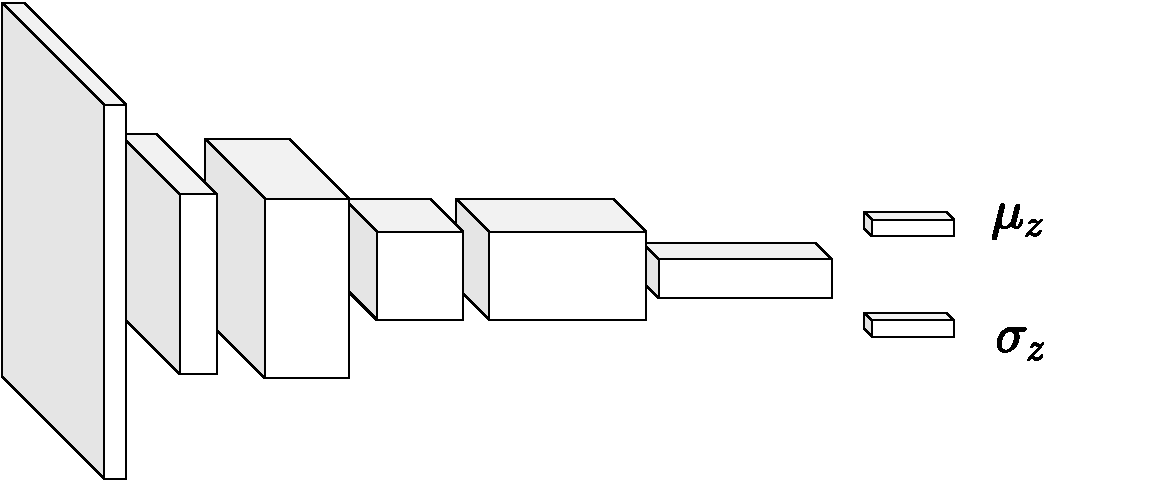
\includegraphics[width=0.9\textwidth]{networks_vae_recognition}
  \end{figure}

  \note{
    \begin{itemize}
      \item Let's just assume the $p(z)$ is gaussian distributed.
      \item And let's additionally assume all elements of $z$ are independent.
      \item To approximate $q(z|x)$ we learn a mapping with a neural net.
      \item This is the encoder part of the variational autoencoder (sometimes called recognition model).
    \end{itemize}
  }

\end{frame}


\begin{frame}{Variational Autoencoder (VAE)}

  \begin{align*}
    MSE(x,\hat{x})
  \end{align*}

  \begin{figure}
    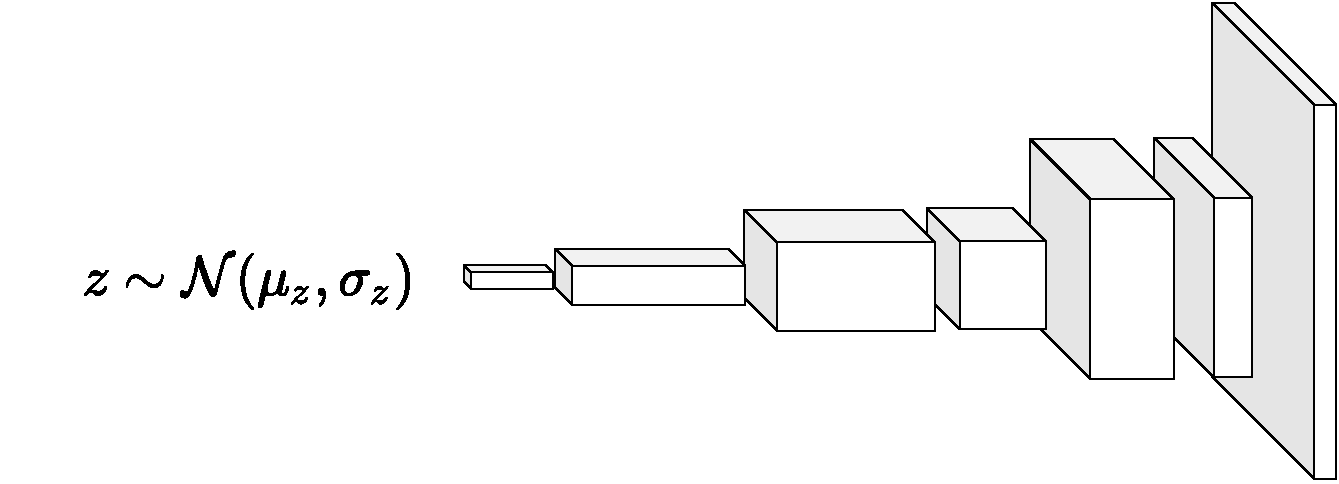
\includegraphics[width=0.9\textwidth]{networks_vae_generator}
  \end{figure}

  \note{
    \begin{itemize}
      \item minimize $MSE(x,\hat{x})$ to maximize $E_{q(z|x)} \log p(x|z)$
      \item This is the decoder part of the variational autoencoder (sometimes called generator model).
    \end{itemize}
  }

\end{frame}


\begin{frame}{Variational Autoencoder (VAE)}

  \begin{figure}
    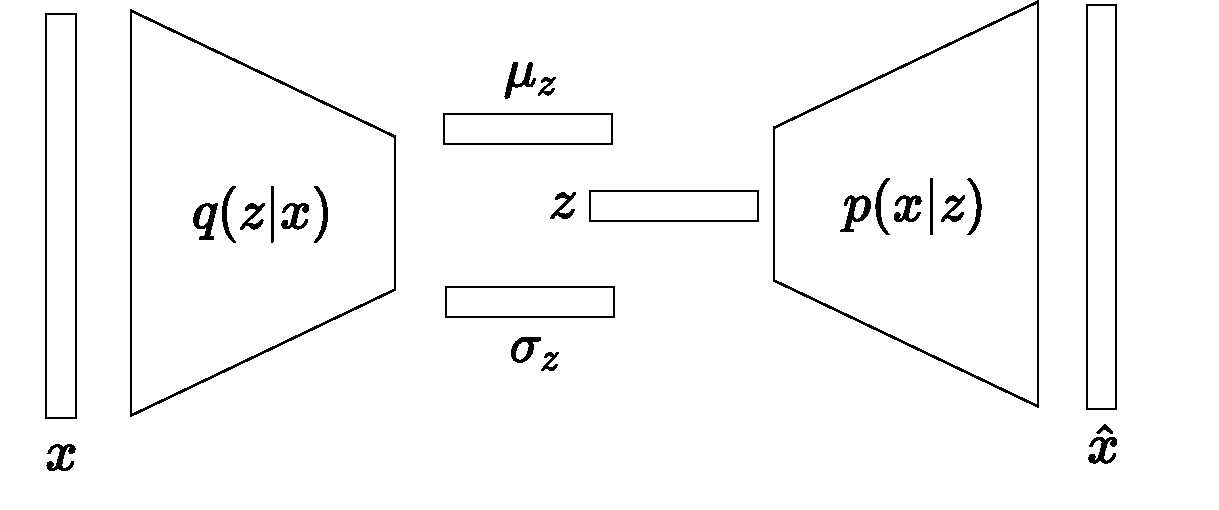
\includegraphics[width=0.9\textwidth]{networks_vae_full}
  \end{figure}

  \note{
    \begin{itemize}
      \item Full VAE architecture for training.
    \end{itemize}
  }

\end{frame}


\begin{frame}{VAE: Reparameterization Trick}

  \begin{align*}
    z = \mu_{z}+\epsilon\sigma_{z}~with~\epsilon ~ \mathcal{N}(0, 1)
  \end{align*}

  \begin{figure}
    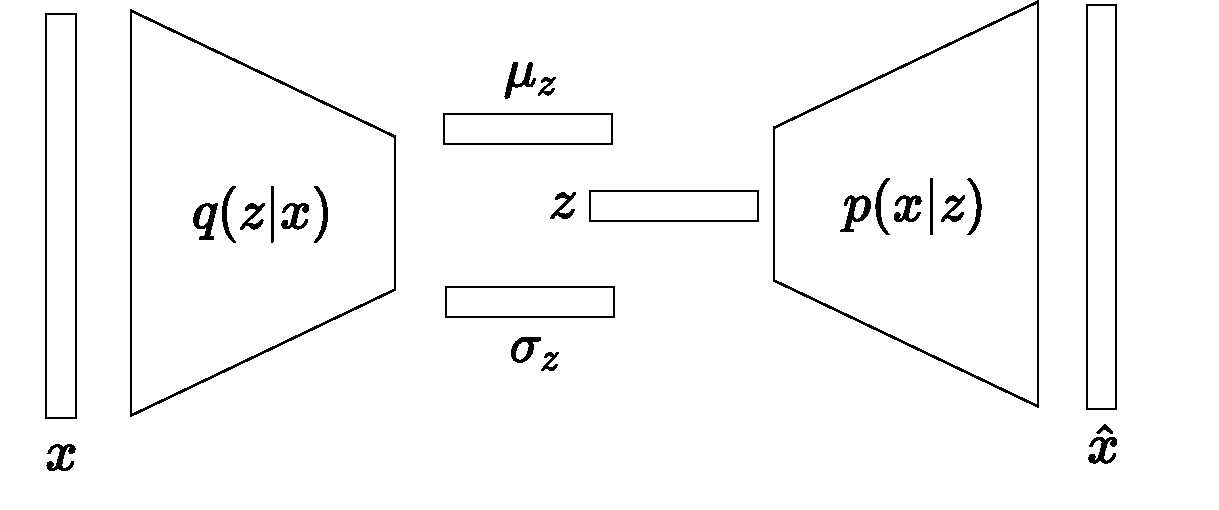
\includegraphics[width=0.9\textwidth]{networks_vae_full}
  \end{figure}

  \note{
    \begin{itemize}
      \item We cannot backpropagate through $z \sim \mathcal{N}(\mu_{z}, \sigma_{z})$
      \item Therefor we set to $z=\mu_{z}+\epsilon\sigma_{z}$ with $\epsilon ~ \mathcal{N}(0, 1)$
      \item This is called the reparameterization trick.
    \end{itemize}
  }

\end{frame}


\begin{frame}{Variational Autoencoder (VAE)}

  \begin{figure}
    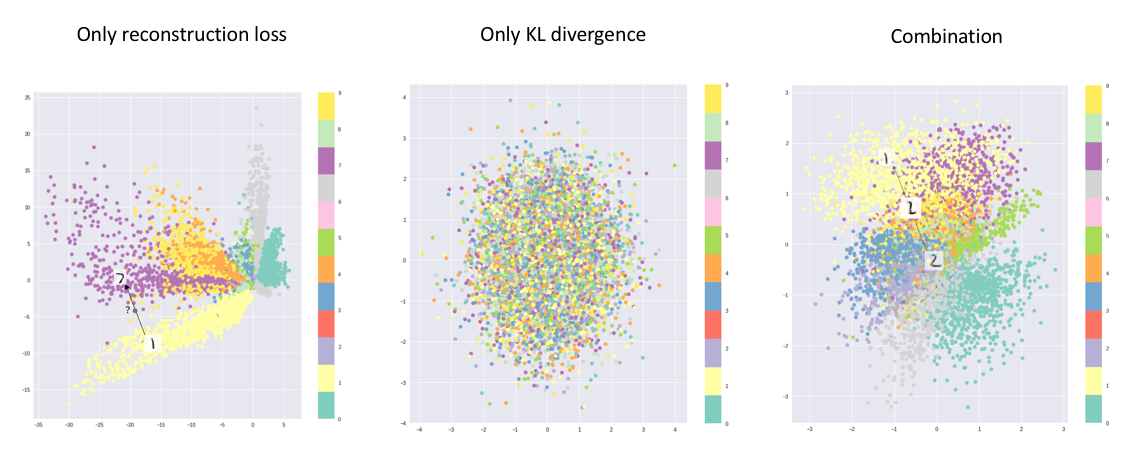
\includegraphics[width=0.9\textwidth]{vae_zviz}
  \end{figure}

  \note{
    \begin{itemize}
      \item At test time we draw $z$ from $p(z)=\mathcal{N}(0, 1)$.
      \item Enforcing $KL(q(z|x)||p(z))$ leads to a smooth latent state.
      \item Image from \url{https://towardsdatascience.com/intuitively-understanding-variational-autoencoders-1bfe67eb5daf}
    \end{itemize}
  }

\end{frame}


\begin{frame}{Variational Autoencoder (VAE)}

  \begin{figure}
    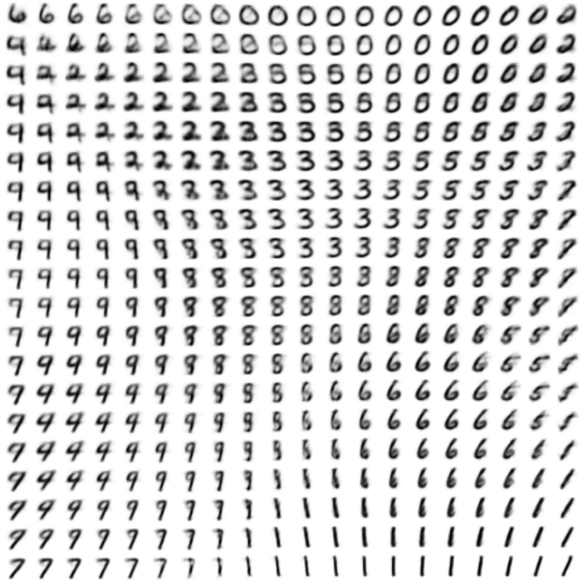
\includegraphics[width=0.5\textwidth]{vae_mnist}
  \end{figure}

  \note{
    \begin{itemize}
      \item A VAE trained to generate MNIST digits.
      \item A grid in the latent space leads to consistent generations in pixelspace.
      \item Image from Auto-Encoding Variational Bayes, Kingma \& Welling, ICLR 2014
    \end{itemize}
  }

\end{frame}



\begin{frame}{Adversarial Learning}

  \begin{columns}
    \begin{column}{0.25\textwidth}
      \begin{figure}
        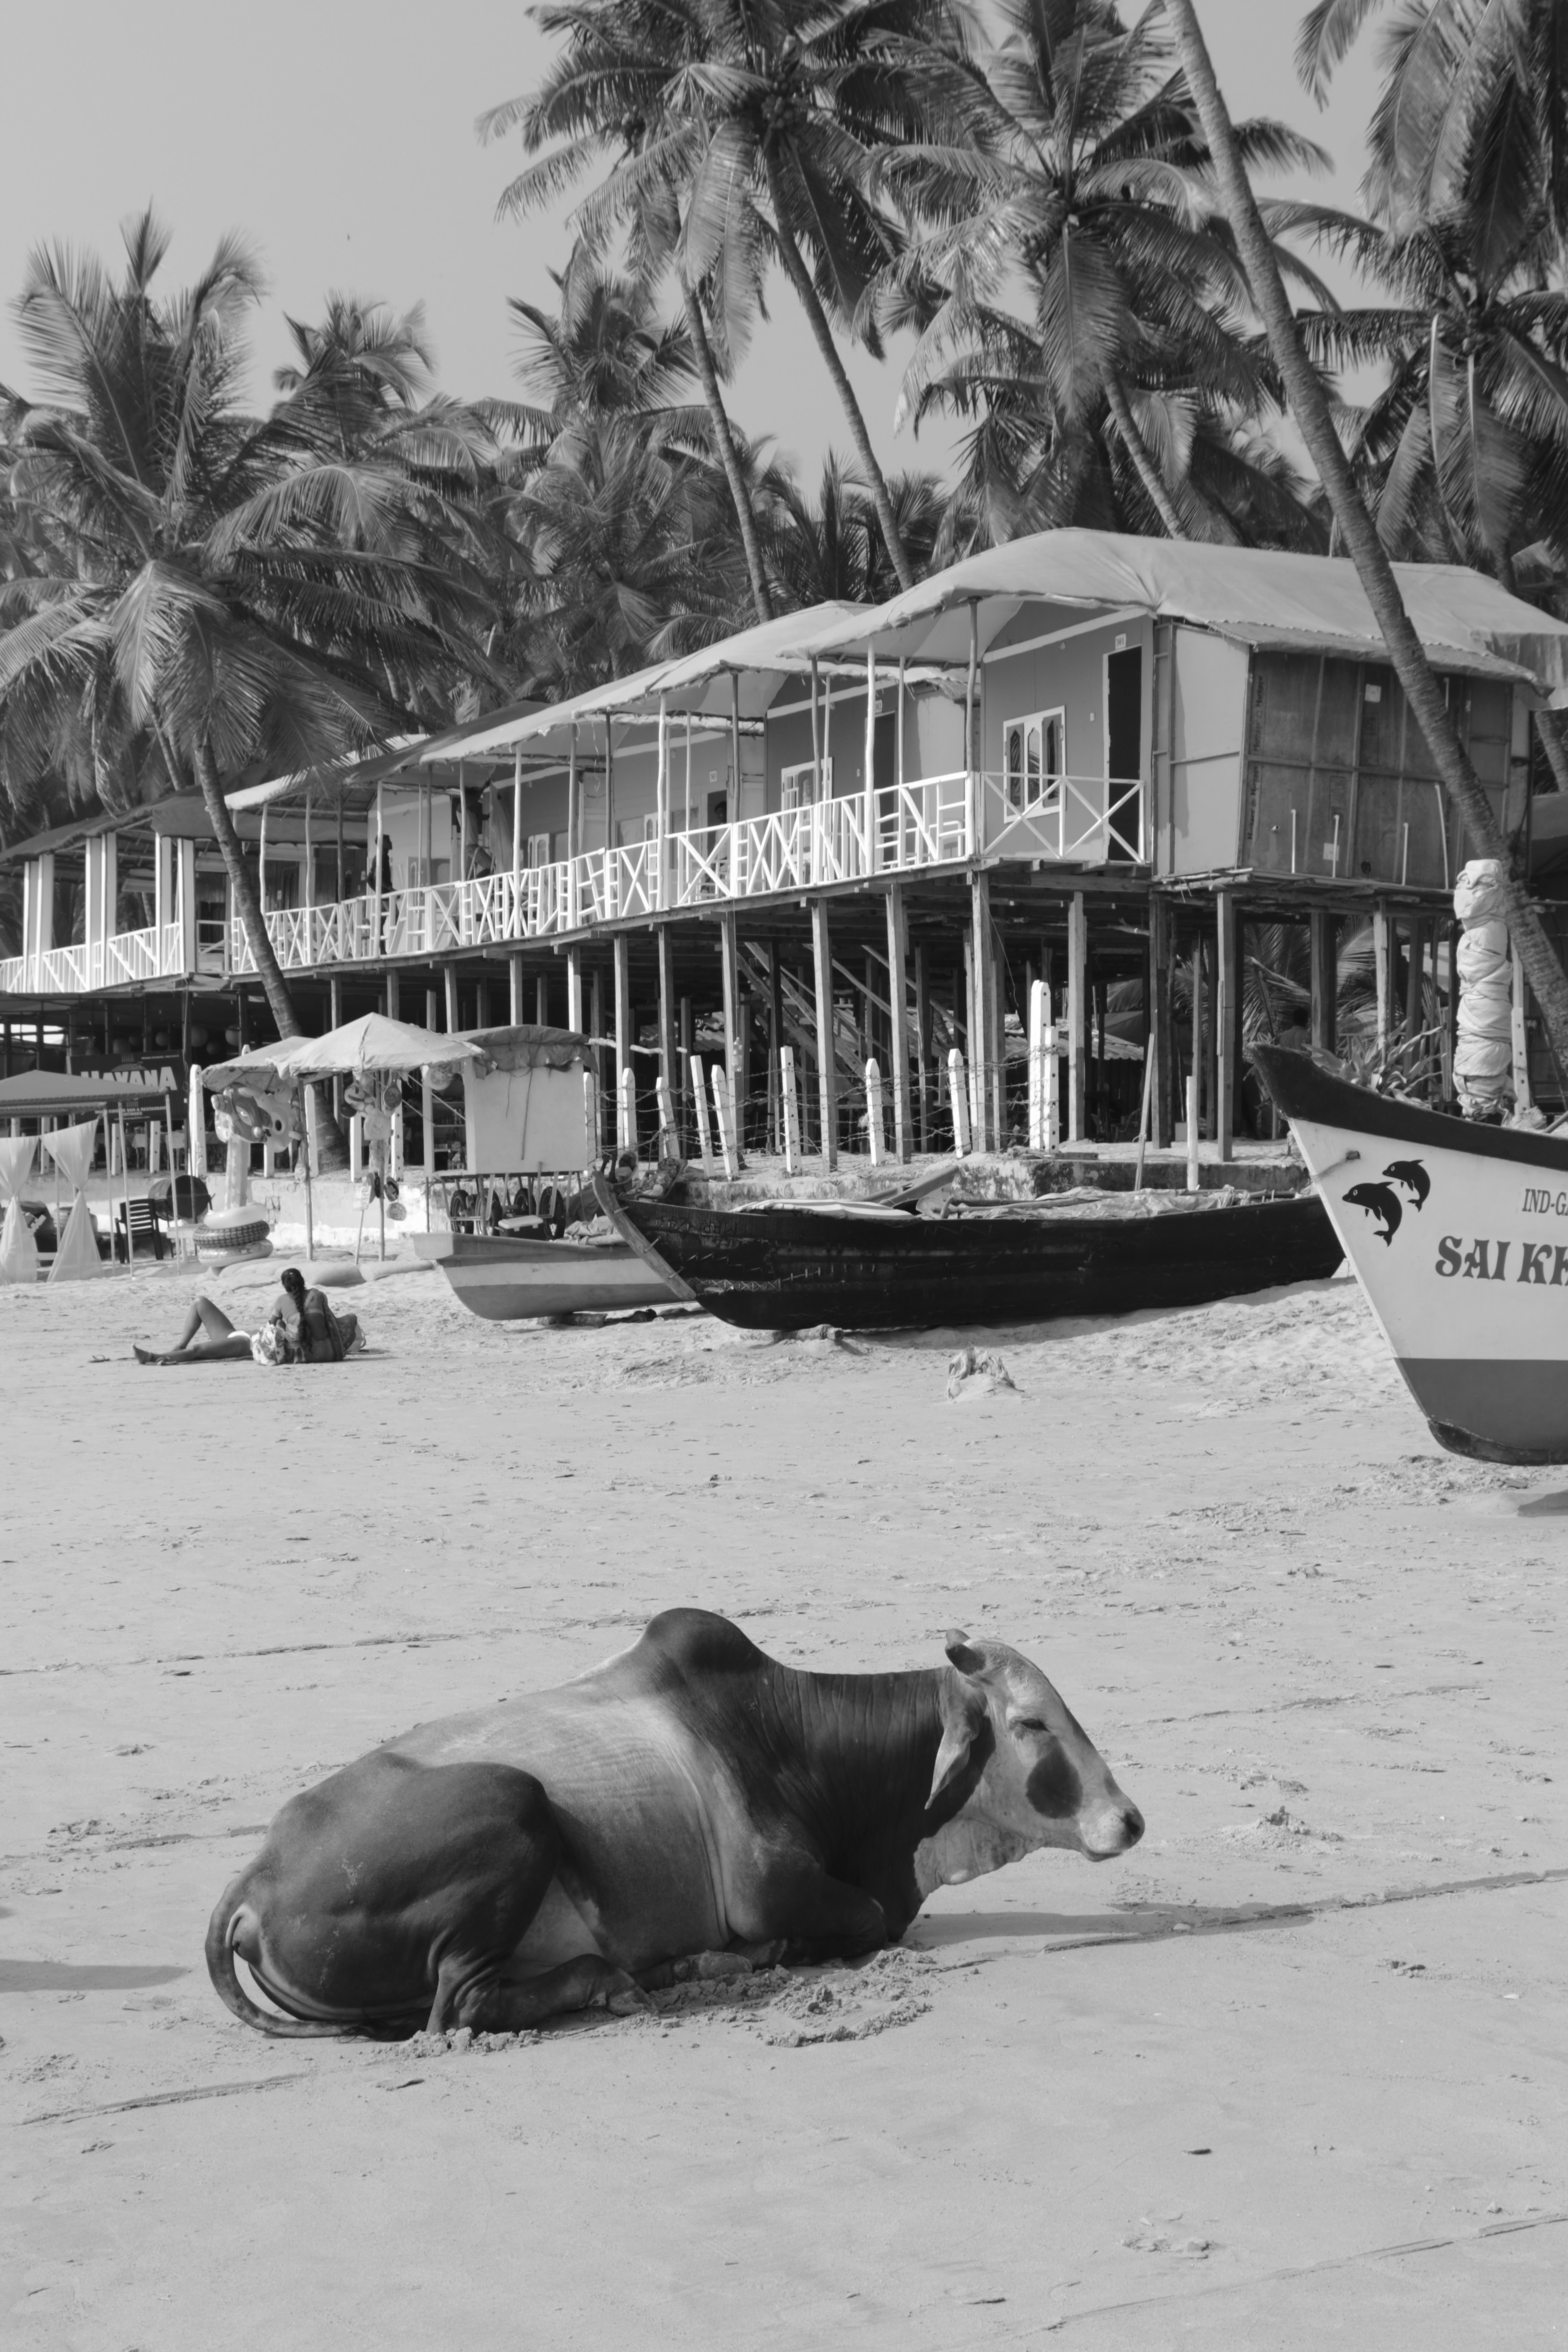
\includegraphics[width=0.9\textwidth]{cow_grey}
      \end{figure}
    \end{column}
    \begin{column}{0.45\textwidth}
      \begin{figure}
        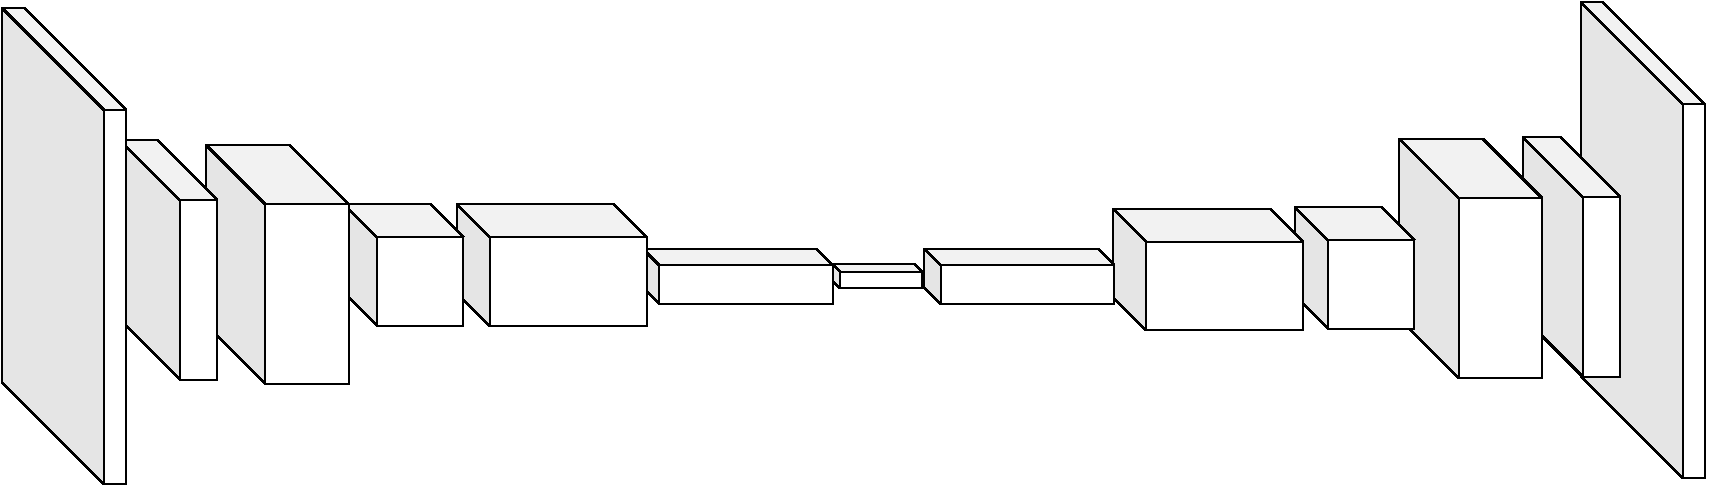
\includegraphics[width=1.0\textwidth]{networks_autoencoder}
      \end{figure}
    \end{column}
    \begin{column}{0.25\textwidth}
      \begin{figure}
        \includegraphics[width=0.9\textwidth]{cow_orig}
      \end{figure}
    \end{column}
  \end{columns}

  \note{
    \begin{itemize}
      \item If we have a generated image (e.g. from the VAE or from colorizing a grey scale image), we do not actually care if the image is exactly the same as the input image.
      \item We just want it to be realistic. But the MSE forces the output to be the same as the reference.
    \end{itemize}
  }
\end{frame}


\begin{frame}{Adversarial Learning}

  \begin{columns}
    \begin{column}{0.95\textwidth}
      \begin{figure}
        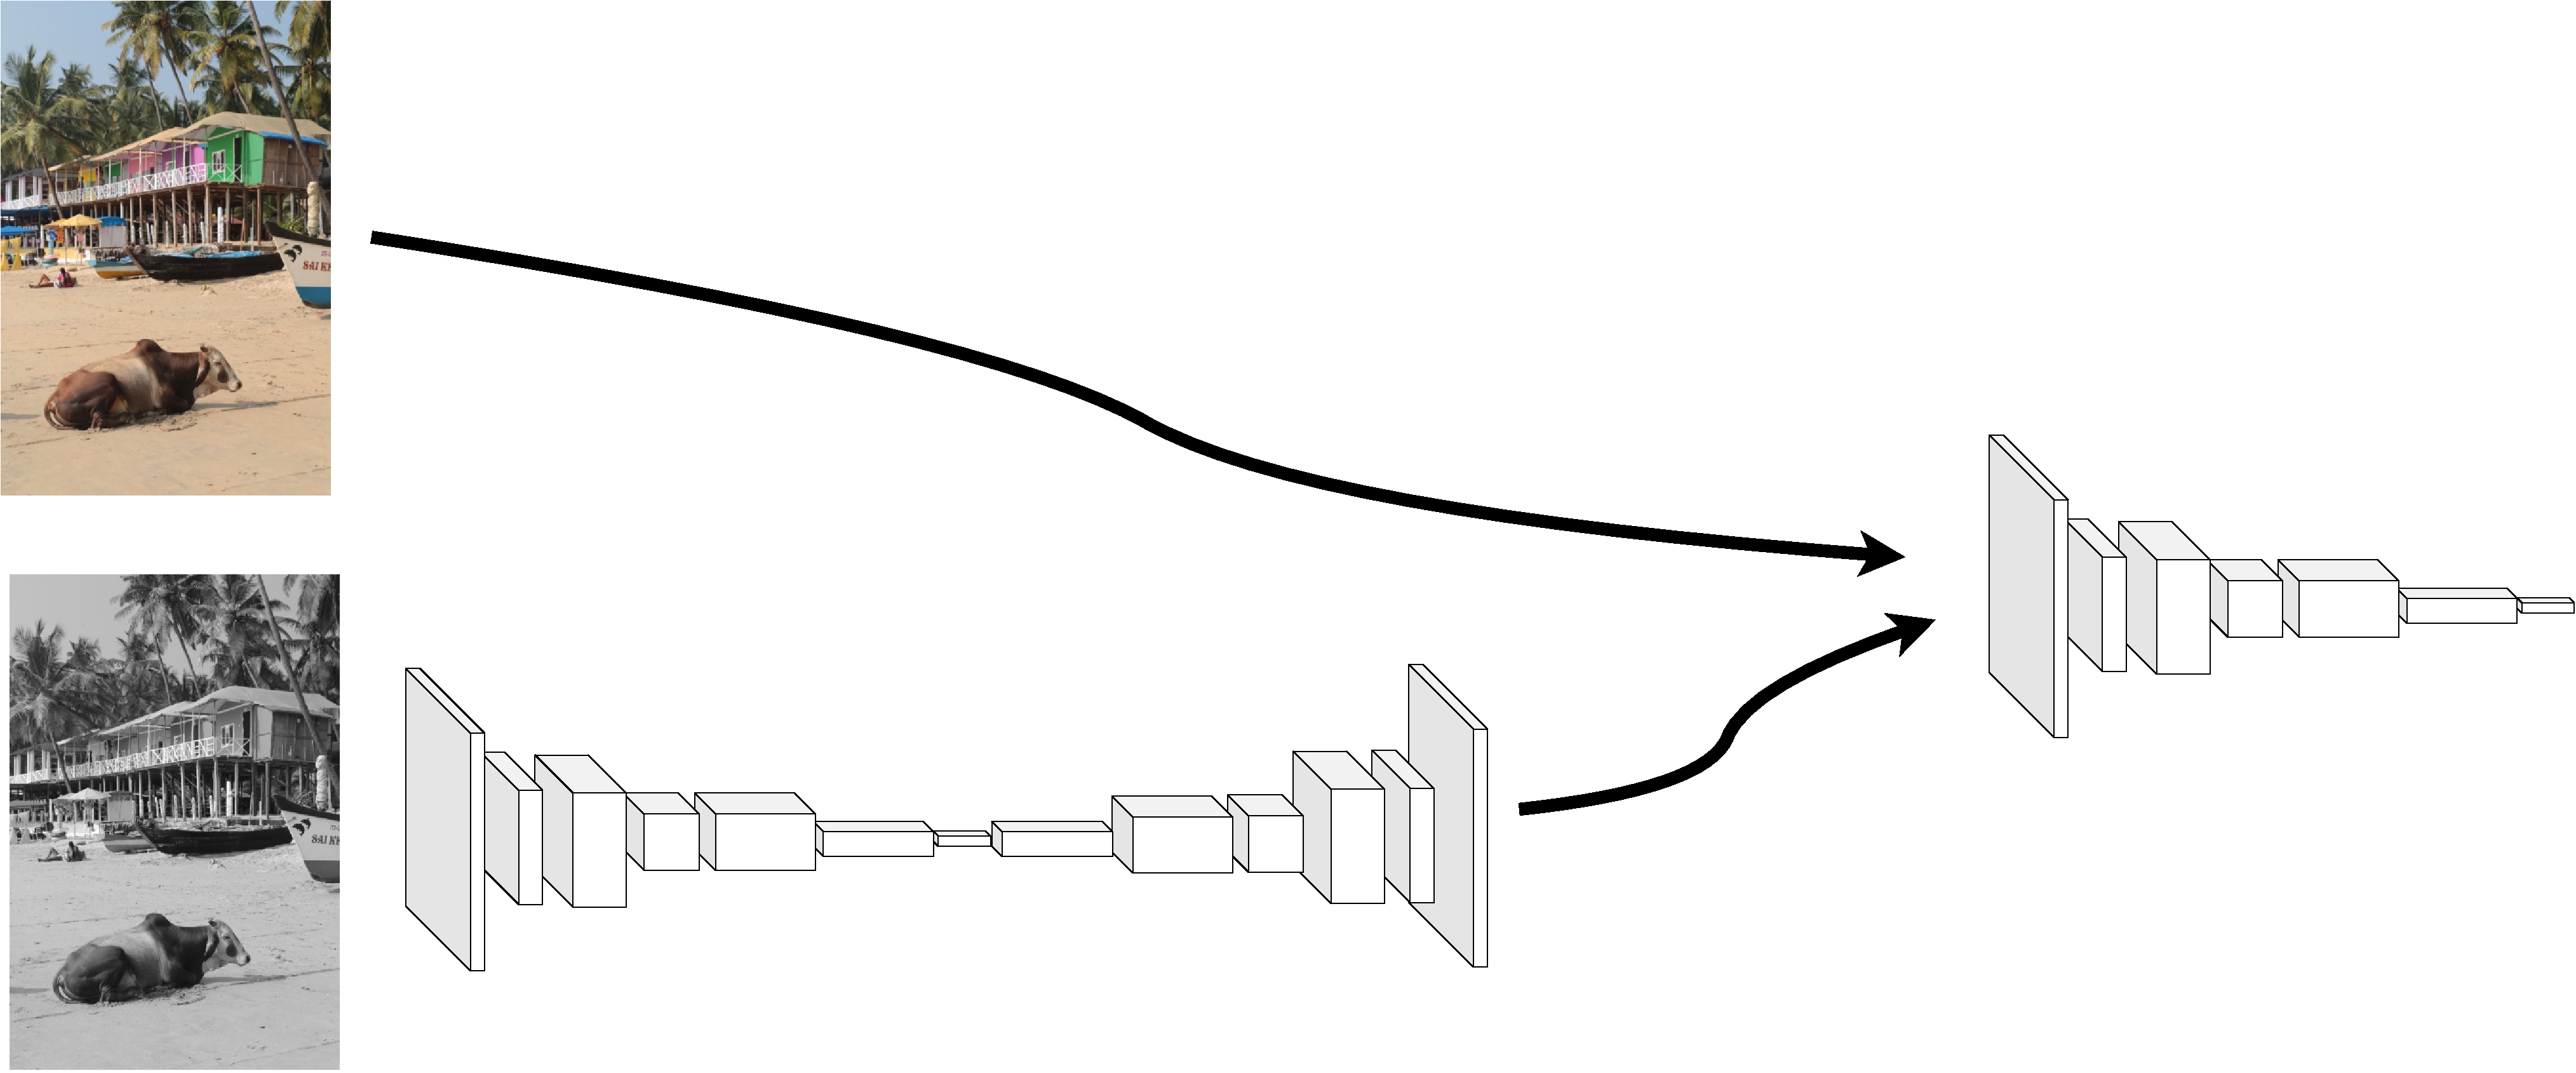
\includegraphics[width=.99\textwidth]{networks_adversarial_loss}
      \end{figure}
    \end{column}
    \begin{column}{0.05\textwidth}
      \begin{align*}
        Fake/Real
      \end{align*}
    \end{column}
  \end{columns}

  \note{
    \begin{itemize}
      \item Instead of formulating a good error measurement ourselves, we can train a classifier to distinguish between a real image and a generated (fake) image.
      \item This way we do not measure if the image looks similar to the original but only if the image looks realistic.
    \end{itemize}
  }
\end{frame}


\begin{frame}{Adversarial Learning}

  \begin{columns}
    \begin{column}{0.95\textwidth}
      \begin{figure}
        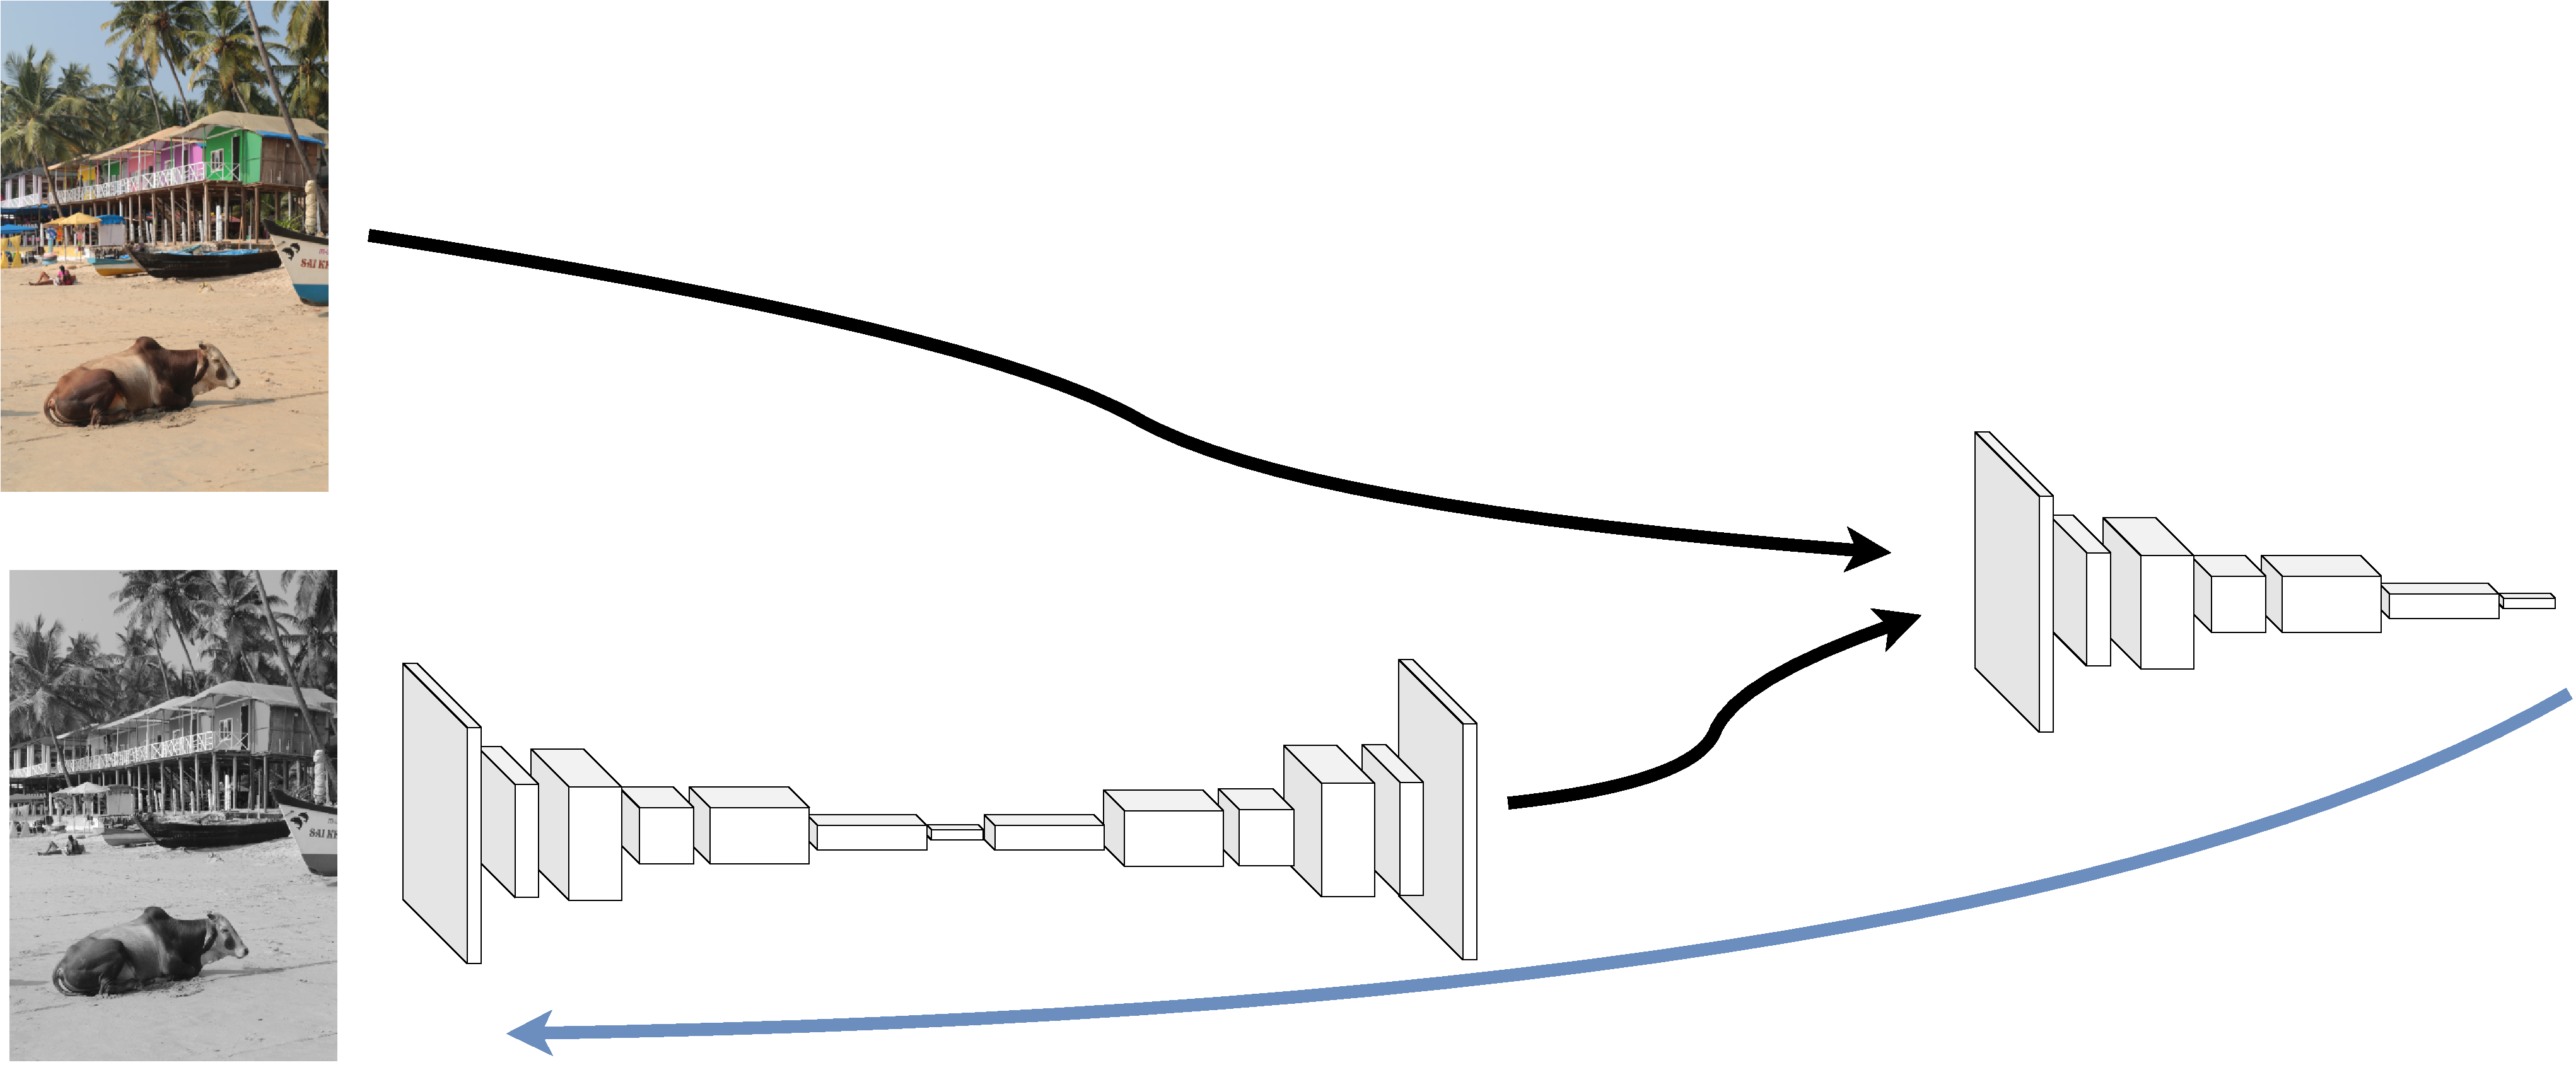
\includegraphics[width=.99\textwidth]{networks_adversarial_loss_gradient}
      \end{figure}
    \end{column}
    \begin{column}{0.05\textwidth}
      \begin{align*}
        Fake/Real
      \end{align*}
    \end{column}
  \end{columns}

  \note{
    \begin{itemize}
      \item After training the classifier (discriminator), we can backpropagate the negative gradient of the discriminator into the generator network.
      \item This way we train the generator to become a better forger. We can train both networks alternatingly, leading to ever better generator and discriminator.
    \end{itemize}
  }
\end{frame}


\begin{frame}{Generative Adversarial Networks}

  \begin{columns}
    \begin{column}{0.95\textwidth}
      \begin{figure}
        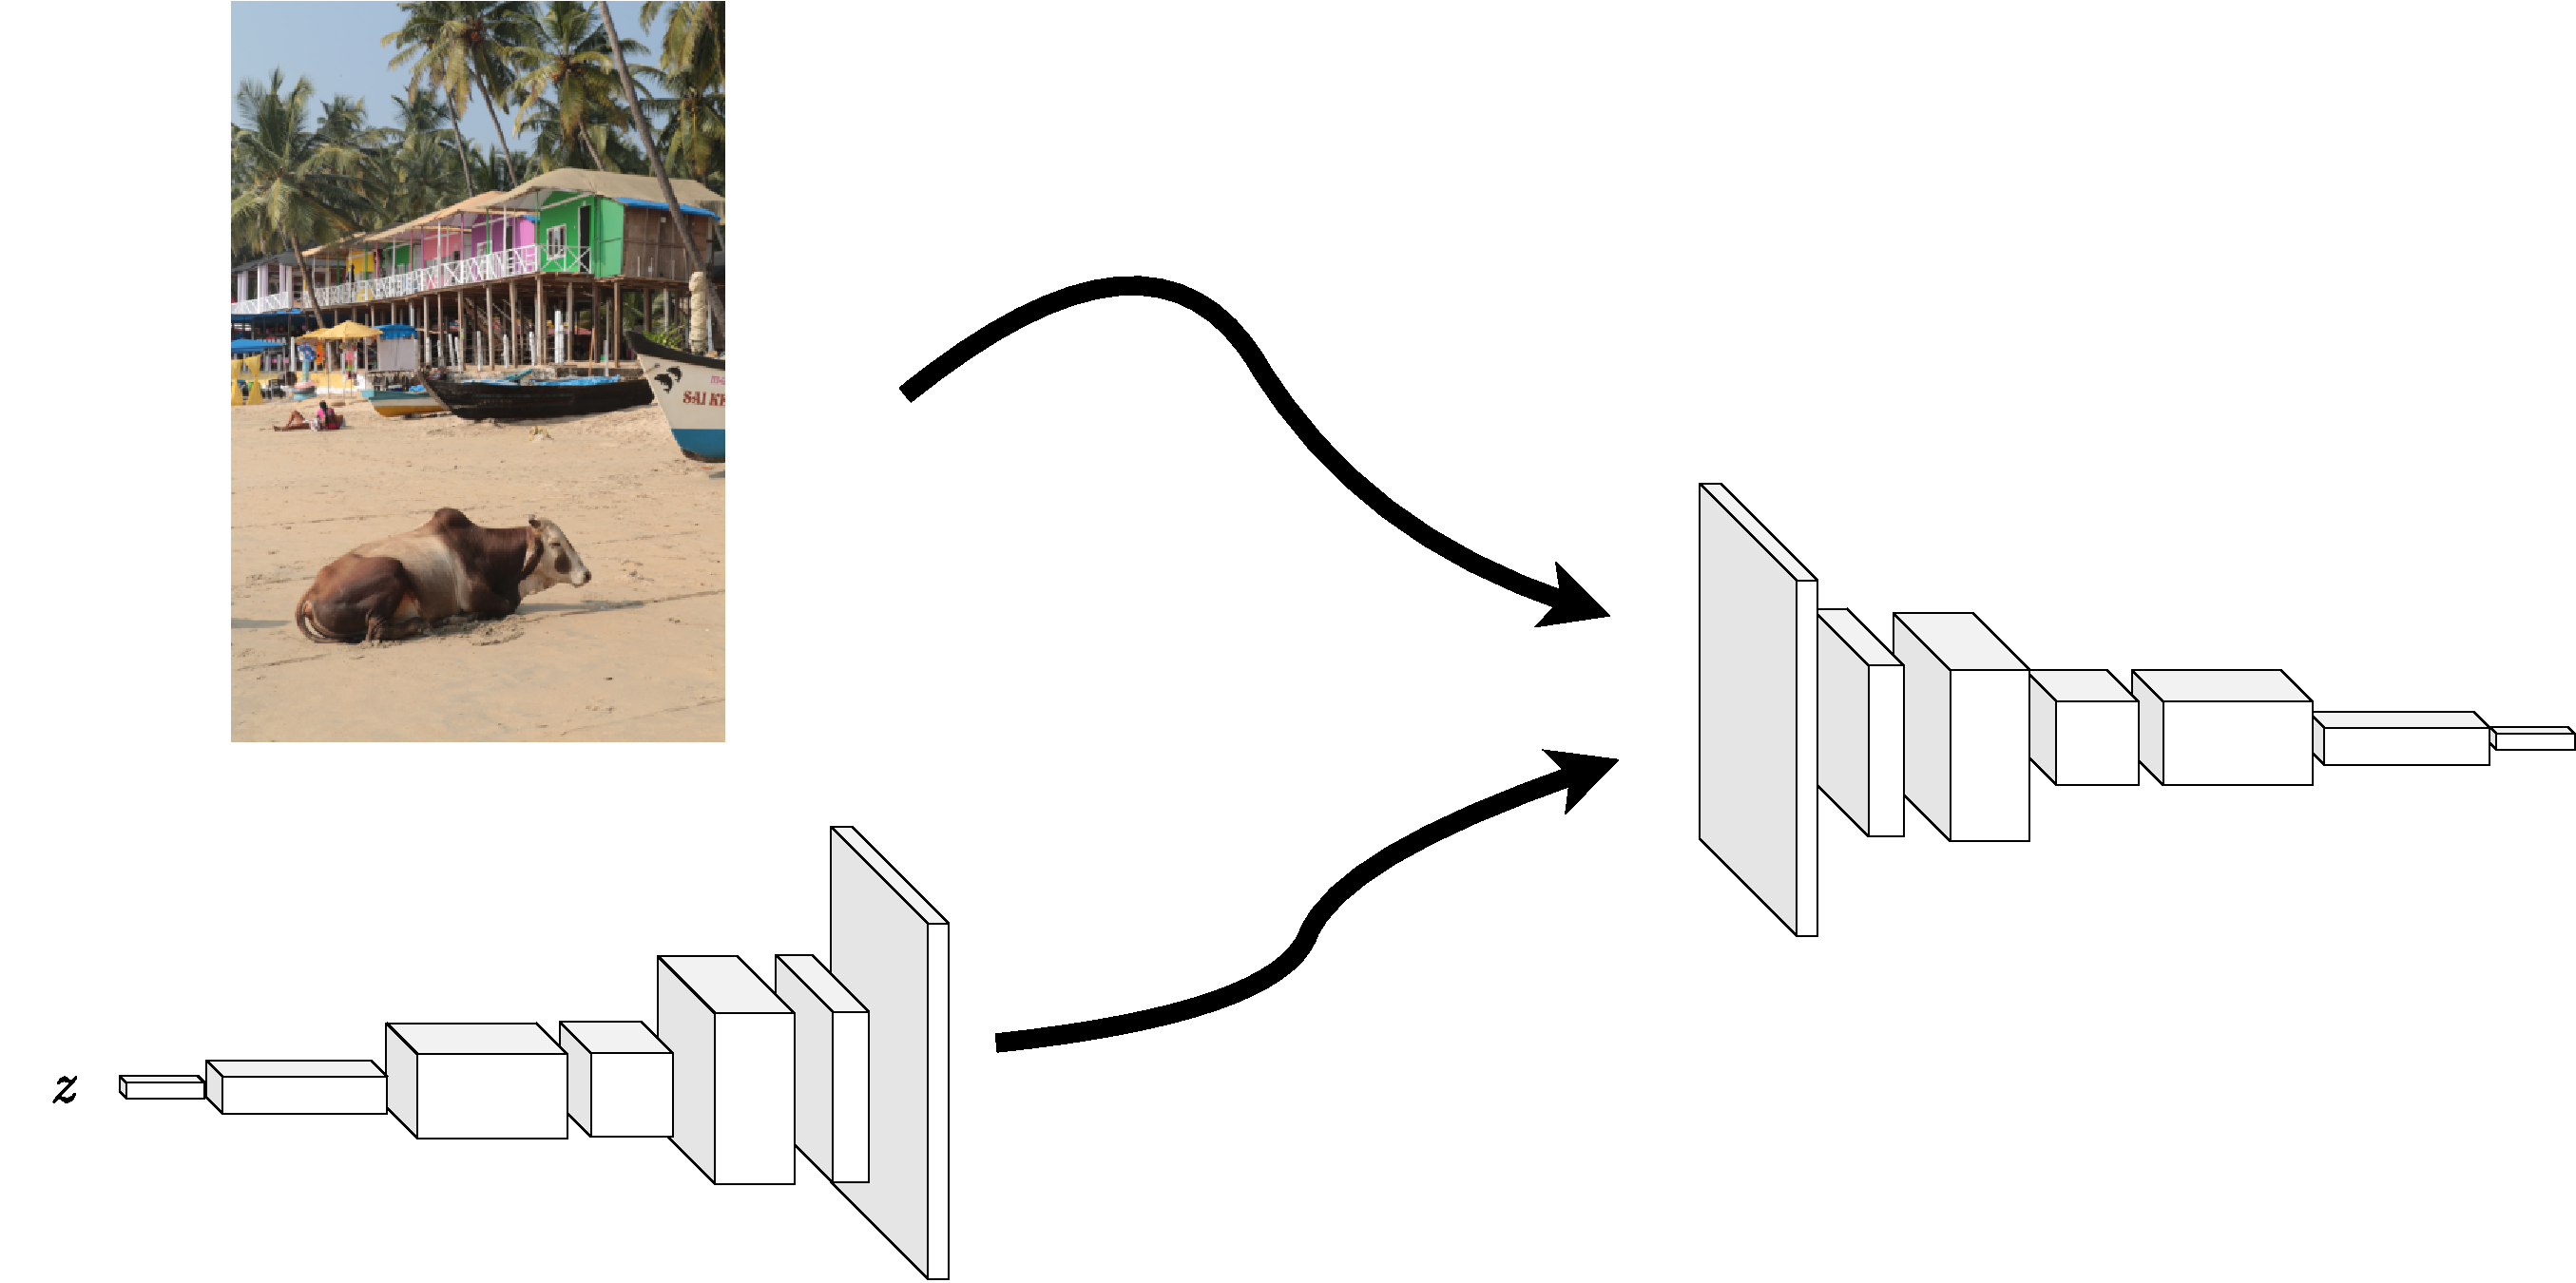
\includegraphics[width=0.99\textwidth]{networks_gan}
      \end{figure}
    \end{column}
    \begin{column}{0.05\textwidth}
      \begin{align*}
        Fake/Real
      \end{align*}
    \end{column}
  \end{columns}

  \note{
    \begin{itemize}
      \item Instead of generating an image from an input encoding, we can also just generate an image from a random vector.
      \item This way the generator learns to map the input distribution $p(z)$ to the data distribution $p(x)$.
      \item The discriminator learns to distinguish if an image $x$ is within $p(x)$ or out of distribution.
    \end{itemize}
  }
\end{frame}


\begin{frame}{Generative Adversarial Networks}

  \begin{align*}
    \min_{\theta_{g}}\max_{\theta_{d}} [ E_{x\sim p_{data}}\log D_{\theta}(x) + E_{z\sim p(z)}\log(1-D_{\theta_{d}}(G_{\theta_{g}}(z)))]
  \end{align*}

  \note{
    \begin{itemize}
      \item Generative Adversarial Networks, Goodfellow et al., NeurIPS 2014
      \item Training of the pair of networks is a mini-max game.
    \end{itemize}
  }
\end{frame}


\begin{frame}{Deep Convolutional GANs}

  \begin{figure}
    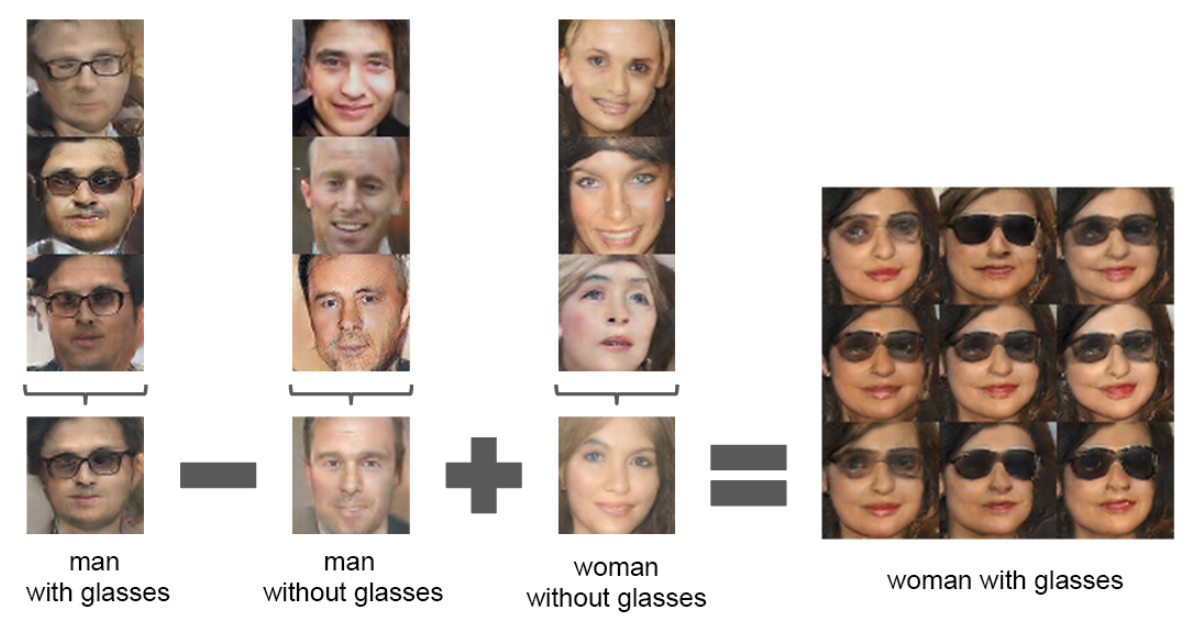
\includegraphics[width=0.8\textwidth]{dcgan_arithmetic}
  \end{figure}

  \note{
    \begin{itemize}
      \item Unsupervised Representation Learning with Deep Convolutional Generative Adversarial Networks, Radford et al.,  ICLR 2016
      \item Paper also uses discriminator features for image classification and lists design guidelines for ConvNet architectures for GANS.
    \end{itemize}
  }

\end{frame}


\begin{frame}{Many improvements ...}

  \begin{itemize}
    \item Wasserstein GAN, Arjovsky et al., 2017
    \item Improved Training of Wasserstein GANs, Gulrajani et al., 2017
    \item Progressive Growing of GANs for Improved Quality, Stability, and Variation, Karras et al., 2017
  \end{itemize}

  \note{
    \begin{itemize}
      \item GANs are hard to train and improvements to training stability were very important.
    \end{itemize}
  }

\end{frame}


\begin{frame}{GAN Zoo}

  \begin{figure}
    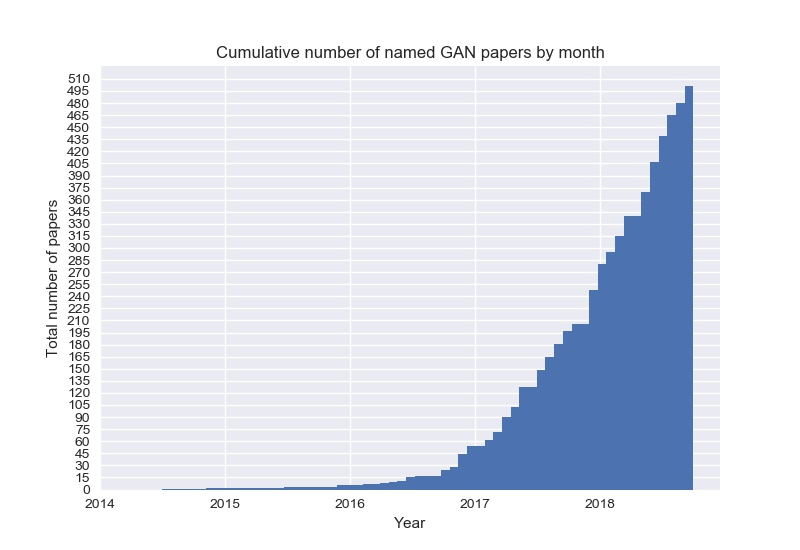
\includegraphics[width=0.8\textwidth]{cumulative_gans}
  \end{figure}

  \note{
    \begin{itemize}
      \item \url{https://github.com/hindupuravinash/the-gan-zoo}
    \end{itemize}
  }

\end{frame}


\begin{frame}{BigGAN}

  \begin{figure}
    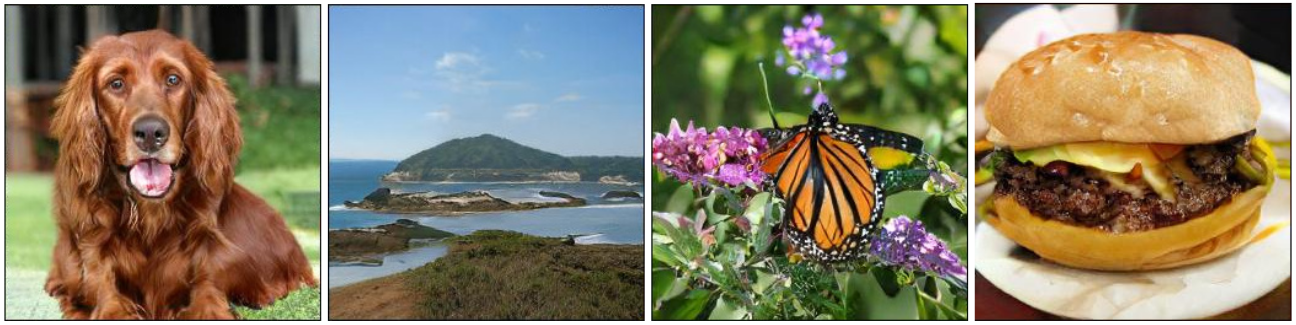
\includegraphics[width=0.9\textwidth]{biggan}
  \end{figure}

  \note{
    \begin{itemize}
      \item Large Scale GAN Training for High Fidelity Natural Image Synthesis, Brock et al., 2019
      \item Class conditional generation of images.
    \end{itemize}
  }

\end{frame}


\begin{frame}{Taxonomy of generative methods}

  \begin{figure}
    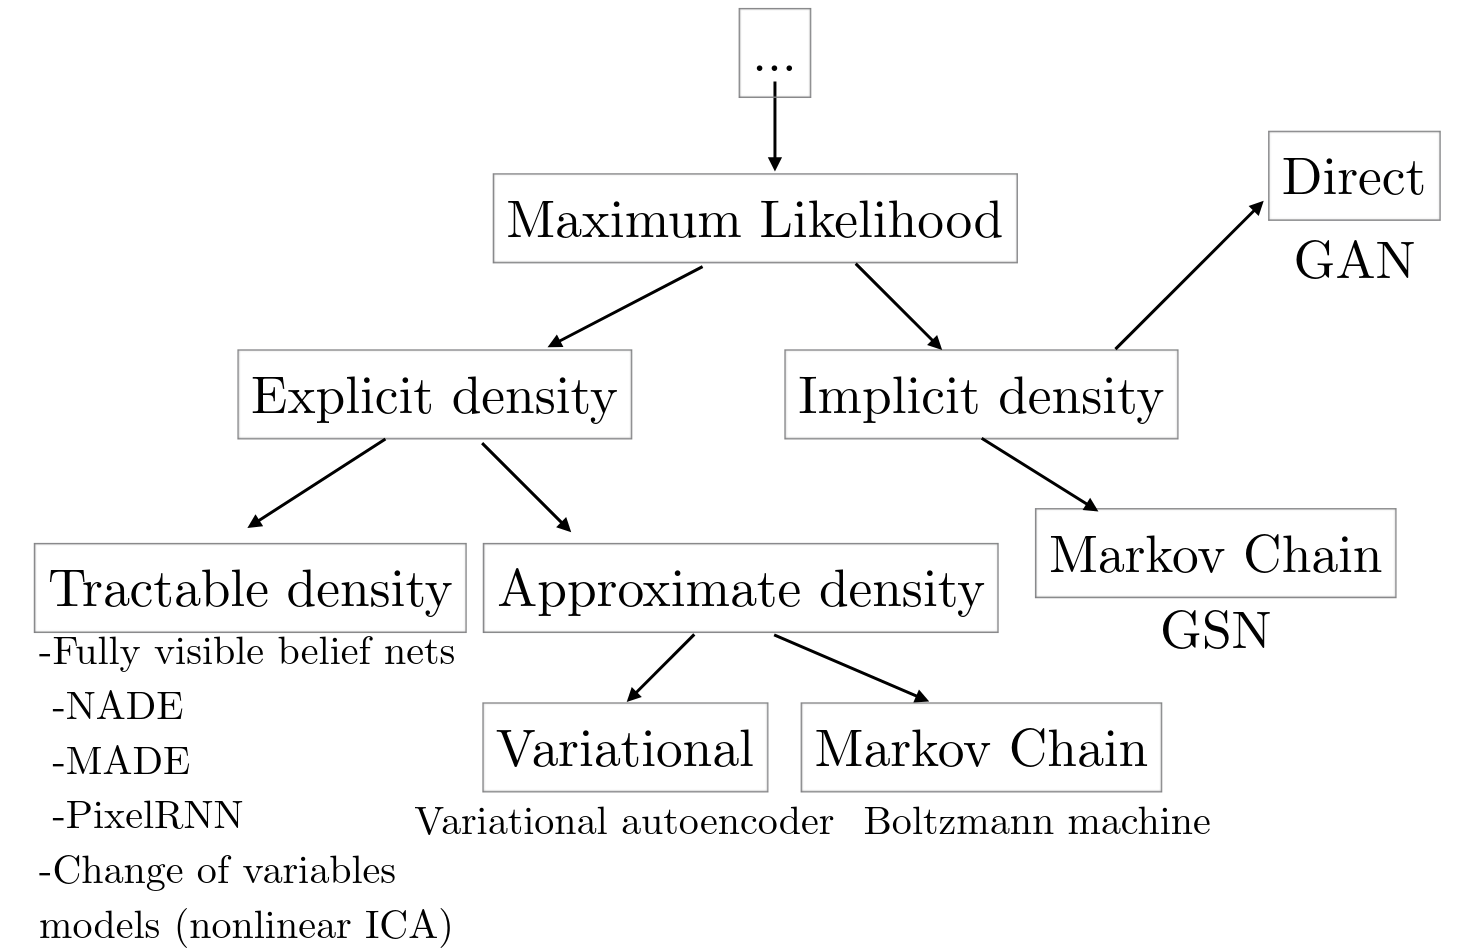
\includegraphics[width=0.9\textwidth]{generative_taxonomy}
  \end{figure}

  \note{
    \begin{itemize}
      \item Image from Tutorial: Generative Adversarial Networks, Godfellow, NeurIPS 2016
    \end{itemize}
  }

\end{frame}
